\documentclass[11pt]{article}
\pdfminorversion=7
\usepackage[utf8]{inputenc}
\usepackage[T1]{fontenc}
\usepackage[english]{babel}
\usepackage{lmodern,microtype}
\usepackage[a4paper,margin=25mm]{geometry}
\usepackage{amsmath,amssymb,bm,graphicx,booktabs,array,tabularx}
\usepackage[round,authoryear]{natbib}
\usepackage{enumitem,placeins,xcolor}
\usepackage[colorlinks=true,linkcolor=blue!45!black,citecolor=blue!45!black,urlcolor=blue!45!black]{hyperref}
\usepackage{caption,xurl}
\captionsetup{font=small,labelfont=bf}
\setlength{\parskip}{4pt}
\setlength{\parindent}{1em}
\setlength{\emergencystretch}{2em}
\setlength{\textfloatsep}{16pt}
\renewcommand{\topfraction}{0.9}
\renewcommand{\bottomfraction}{0.8}
\renewcommand{\textfraction}{0.08}
\renewcommand{\floatpagefraction}{0.45}
\setcounter{topnumber}{3}
\setcounter{totalnumber}{5}
\raggedbottom
\graphicspath{{figures/}{legacy_figures/}}
\newcommand{\E}{\operatorname{E}}
\newcommand{\Var}{\operatorname{Var}}
\newcommand{\diag}{\operatorname{diag}}

\renewcommand{\thesection}{S\arabic{section}}
\renewcommand{\thetable}{S\arabic{table}}
\renewcommand{\thefigure}{S\arabic{figure}}
\renewcommand{\theequation}{S\arabic{equation}}
\title{Supplementary material\\Bayesian spectral selection for road-segment crash counts}
\author{Danna L. Cruz-Reyes, Juan Sosa and Carlos A. Mart\'inez}
\date{}
\begin{document}\maketitle
\section{Evidence versions and computational scope}
This supplement separates newly fitted empirical specifications from a historical simulation experiment supplied with the preceding manuscript. Sections S1--S4 document the revised empirical analysis. The historical section retains the earlier simulation design and reported summaries, explicitly without treating them as a validation of the revised ordered mixture prior or its adjusted empirical fits. The simulation was not rerun during this revision.

The revised main-text analysis uses the retained supports of 2,540 Barcelona and 6,079 Bogot\'a segments, the ordered slab variance $0.05^2+\tau^2/(1-0.9\lambda_j)$, an independent $N(0,5^2)$ intercept prior and four-chain inference. The historical manuscript used the unaugmented slab variance $\tau^2/(1-0.9\lambda_j)$ and different empirical preprocessing and computational specifications. The current and historical versions must not be combined into a single model-performance claim.

The computational archive \texttt{modelos\_espectrales\_resultados.zip} contains prepared inputs, source code, posterior core-parameter draws and numerical summaries for the 20 revised specifications. Complete chain CSV files are retained locally and their paths recorded in each fit's metadata; those local paths are not a public archive. Dataset hashes, code hashes and package versions identify the available computation. Public deposition and source-event reconciliation remain author tasks.

\section{Recorded categories and coefficients}
Unknown categories are nuisance labels for incomplete attribute recording. They are not interpreted as physically absent lanes or surface. Another recorded surface tag includes generic \texttt{paved}; it need not mean absence of asphalt. The single recorded lane count of 22 in Bogot\'a was treated as unknown. The following counts refer to the retained analytical samples.
\begin{table}[!htbp]\centering\small
\caption{Recorded attribute categories on the retained support.}
\begin{tabular}{llrr}\toprule Attribute & Category & Barcelona & Bogot\'a\\\midrule
Road class & residential & 932 & 2658 \\
Road class & tertiary & 530 & 1377 \\
Road class & secondary & 800 & 1282 \\
Road class & primary & 278 & 762 \\
Lanes & two & 659 & 4260 \\
Lanes & one & 298 & 461 \\
Lanes & three\_plus & 1153 & 860 \\
Lanes & unknown & 430 & 498 \\
Surface tag & asphalt & 2380 & 5336 \\
Surface tag & other\_recorded & 22 & 583 \\
Surface tag & unknown & 138 & 160 \\
\bottomrule\end{tabular}\end{table}
\FloatBarrier
\begin{table}[!htbp]\centering\small
\caption{Complete conditional count-ratio summaries for recorded attributes in the mixture spectral model with estimated length. Intervals are marginal 90\% posterior intervals. Unknown-category coefficients are retained for reproducibility but have no infrastructure-effect interpretation.}
\begin{tabular}{llrrr}\toprule Network & Indicator & Median ratio & 5th percentile & 95th percentile\\\midrule
Barcelona & Tertiary road & 1.14 & 0.95 & 1.35 \\
Barcelona & Secondary road & 0.97 & 0.80 & 1.18 \\
Barcelona & Primary road & 1.29 & 1.04 & 1.60 \\
Barcelona & One lane & 0.84 & 0.69 & 1.03 \\
Barcelona & Three or more lanes & 1.49 & 1.27 & 1.74 \\
Barcelona & Unknown lane count & 0.74 & 0.60 & 0.91 \\
Barcelona & Other surface tag & 0.86 & 0.52 & 1.48 \\
Barcelona & Unknown surface & 0.71 & 0.55 & 0.92 \\
Bogot\'a & Tertiary road & 1.95 & 1.78 & 2.13 \\
Bogot\'a & Secondary road & 2.59 & 2.36 & 2.84 \\
Bogot\'a & Primary road & 3.73 & 3.35 & 4.17 \\
Bogot\'a & One lane & 1.07 & 0.95 & 1.20 \\
Bogot\'a & Three or more lanes & 1.29 & 1.17 & 1.43 \\
Bogot\'a & Unknown lane count & 0.55 & 0.48 & 0.63 \\
Bogot\'a & Other surface tag & 0.82 & 0.73 & 0.92 \\
Bogot\'a & Unknown surface & 1.19 & 0.97 & 1.47 \\
\bottomrule\end{tabular}\end{table}
\FloatBarrier
\section{Sampling and predictive diagnostics}
The joint operational criterion requires no divergent transitions, no depth saturation, maximum rank-normalized $\widehat R\leq1.01$, minimum bulk ESS of 400 and minimum E-BFMI of 0.3. The four BYM2-type runs were repeated with 2,000 warm-up and 2,000 sampling iterations in each of four chains. All retained fits have zero divergences and depth saturations. Energy warnings persist in the BYM2-type fits; successful completion is not a statement of adequate posterior exploration.

In the labels below, N denotes nonspatial NB, D dense spectral, M mixture spectral and B spectral BYM2. U and C impose unit length with no attributes or recorded attributes, respectively; L includes recorded attributes and estimates length. Missing local-effect diagnostics are not relevant to models without those effects.
\begin{table}[!htbp]\centering\small
\caption{Revised empirical fits: core sampler summaries. Minimum E-BFMI is across chains. The main text also requires checks of BYM2 independent effects.}
\begin{tabular}{llrrrrl}\toprule Network & Model & Draws/chain & Max. $\widehat R$ & Min. ESS & Min. E-BFMI & Criterion\\\midrule
Barcelona & B-C & 2000 & 1.006 & 442 & 0.246 & Flagged \\
Barcelona & B-U & 2000 & 1.012 & 386 & 0.203 & Flagged \\
Barcelona & D-C & 1000 & 1.005 & 946 & 0.738 & Pass \\
Barcelona & D-U & 1000 & 1.004 & 752 & 0.666 & Pass \\
Barcelona & N-C & 1000 & 1.002 & 1676 & 0.907 & Pass \\
Barcelona & N-U & 1000 & 1.002 & 1512 & 0.885 & Pass \\
Barcelona & M-C & 1000 & 1.004 & 1456 & 0.966 & Pass \\
Barcelona & M-U & 1000 & 1.004 & 1700 & 0.909 & Pass \\
Barcelona & N-L & 1000 & 1.002 & 1721 & 0.940 & Pass \\
Barcelona & M-L & 1000 & 1.003 & 1529 & 0.904 & Pass \\
Bogot\'a & B-C & 2000 & 1.006 & 376 & 0.191 & Flagged \\
Bogot\'a & B-U & 2000 & 1.004 & 700 & 0.277 & Flagged \\
Bogot\'a & D-C & 1000 & 1.004 & 921 & 0.771 & Pass \\
Bogot\'a & D-U & 1000 & 1.003 & 829 & 0.697 & Pass \\
Bogot\'a & N-C & 1000 & 1.002 & 1820 & 0.973 & Pass \\
Bogot\'a & N-U & 1000 & 1.002 & 1470 & 0.971 & Pass \\
Bogot\'a & M-C & 1000 & 1.004 & 1677 & 0.869 & Pass \\
Bogot\'a & M-U & 1000 & 1.005 & 1660 & 0.881 & Pass \\
Bogot\'a & N-L & 1000 & 1.001 & 1824 & 0.981 & Pass \\
Bogot\'a & M-L & 1000 & 1.003 & 1456 & 0.934 & Pass \\
\bottomrule\end{tabular}\end{table}
\FloatBarrier
\begin{table}[!htbp]\centering\small
\caption{Posterior predictive checks for the mixture spectral L models. Reference intervals use 400 replicated datasets. $p_+$ is the fraction of replicated statistics at least as large as the observed statistic. Extreme values indicate discrepancies, not frequentist significance.}
\begin{tabular}{llrrrl}\toprule Network & Statistic & Observed & Rep. median & 90\% rep. interval & $p_+$\\\midrule
Barcelona & Zero fraction & 0.540 & 0.536 & [0.513, 0.558] & 0.383 \\
Barcelona & Variance & 7.58 & 7.89 & [6.30, 10.68] & 0.595 \\
Barcelona & Maximum & 26.00 & 37.00 & [26.00, 71.10] & 0.958 \\
Barcelona & 99th percentile & 13.00 & 13.00 & [11.61, 15.00] & 0.675 \\
Barcelona & Mean & 1.470 & 1.443 & [1.324, 1.567] & 0.365 \\
Bogot\'a & Zero fraction & 0.283 & 0.249 & [0.237, 0.260] & 0.000 \\
Bogot\'a & Variance & 899.32 & 1034.85 & [795.81, 1406.34] & 0.795 \\
Bogot\'a & Maximum & 815.00 & 700.50 & [443.90, 1353.25] & 0.318 \\
Bogot\'a & 99th percentile & 146.22 & 146.00 & [131.21, 164.23] & 0.490 \\
Bogot\'a & Mean & 13.994 & 13.871 & [13.103, 14.851] & 0.412 \\
\bottomrule\end{tabular}\end{table}
\FloatBarrier
\begin{table}[!htbp]\centering\small
\caption{Residual Moran's $I$ for the estimated-length models. Values use centred Pearson residuals and the reconstructed segment adjacency; the replicated reference is conditional on each draw.}
\begin{tabular}{llrrrl}\toprule Network & Model & Observed median & Rep. median & 90\% rep. interval & $p_+$\\\midrule
Barcelona & N-L & -0.046 & -0.003 & [-0.020, 0.025] & 1.00 \\
Barcelona & M-L & -0.055 & 0.001 & [-0.028, 0.025] & 1.00 \\
Bogot\'a & N-L & 0.118 & 0.000 & [-0.019, 0.016] & 0.00 \\
Bogot\'a & M-L & 0.089 & -0.002 & [-0.013, 0.013] & 0.00 \\
\bottomrule\end{tabular}\end{table}
\FloatBarrier
\section{Field uncertainty and limits of component summaries}
The interval maps below use the mixture spectral L models. Each segment interval is marginal; no simultaneous hotspot decision is implied. The full field combines all coefficients, including coefficients allocated predominantly to the continuous spike. Therefore a field interval can exclude zero on some segments even when no single component has slab-membership probability above 0.5. These are different posterior questions.
\begin{figure}[!htbp]\centering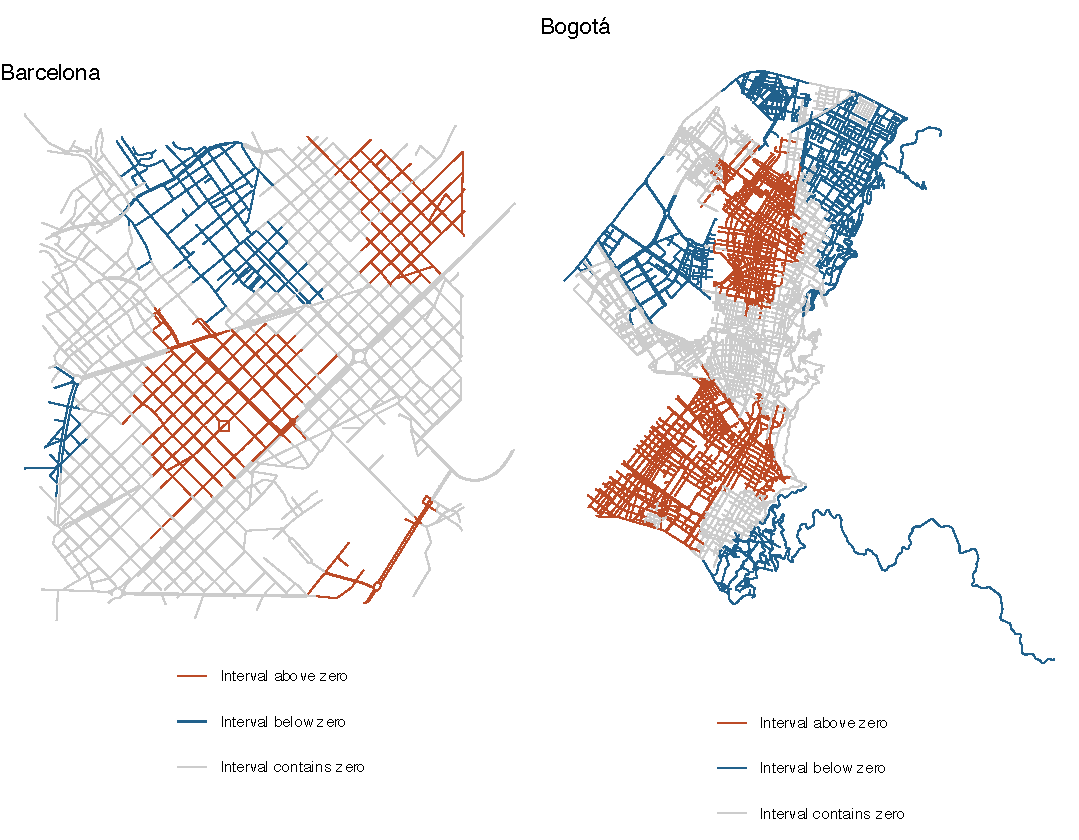
\includegraphics[width=\textwidth]{field_uncertainty.pdf}
\caption{Marginal 90\% intervals for the structured field with recorded attributes and estimated length. Colours indicate interval sign support relative to zero; they are not traffic-adjusted risk categories.}
\end{figure}\FloatBarrier

\section{Historical simulation experiment: preceding specification}
\noindent\textbf{Version boundary.} The following experiment and reported numerical summaries are retained from the supplied preceding manuscript. Its 4,800 fits were not rerun or independently audited here. The prior, empirical preprocessing and two-chain computational budget differ from the revised four-chain applications. References within this historical description to an empirical basis refer to the preceding version, not the revised application. In particular, these results do not validate the ordered slab variance, covariate adjustment or estimated-length models of the main paper.


\label{sec:simulation}

We conducted a simulation study to investigate the conditions under which the legacy sparse spectral model can recover a parsimonious spectral representation of spatial log-frequency on a road network, and to compare its performance with spatial models based on CAR and BYM2 representations. The simulation was designed to distinguish between two related but different objectives: (i) recovery of the latent spatial field and its relevant spectral components, and (ii) out-of-sample prediction of crash counts.

The simulation starts from the spectral representation of two real road-network geometries, corresponding to Barcelona and central Bogotá. For each network, four different data-generating mechanisms were considered, ranging from a setting that exactly favors sparse spectral recovery to deliberately misspecified spatial structures. Three global levels of difficulty were considered for each combination of network and generating mechanism. Each scenario was independently replicated 50 times. Thus, the complete experiment contains $ 2 \text{ networks} \times4 \text{ generating mechanisms} \times 3 \text{ difficulty levels} \times 50 \text{ replications} = 1200 $ simulated datasets. Four competing models are fitted to every simulated dataset, resulting in a total of 4800 Bayesian model fits.

\subsection{Road-network spectral representation}

Let $\mathcal{G}=(\mathcal{V},\mathcal{E})$ denote a road network, where the observational units are the $p=|\mathcal{E}|$ road segments. For each network, the spectral basis retained for the preceding manuscript version was retained for the simulation.

Let

\[
\widetilde U=
\begin{pmatrix}
	\widetilde u_1 & \cdots & \widetilde u_M
\end{pmatrix}
\in\mathbb{R}^{p\times M}
\]

denote the matrix containing the $M$ retained centered and scaled spectral columns, and let $ \lambda_1,\ldots,\lambda_M$ denote the eigenvalues of their uncentered source eigenvectors. The simulation therefore begins at the latent spatial-field level rather than directly at the crash-count level.

For all spectral generating mechanisms, we used $\gamma=0.9$ and defined the spectral weights
\[
w_j
=
\frac{1}{\sqrt{1-\gamma\lambda_j}},
\qquad
j=1,\ldots,M.
\]

These weights determine the relative contribution of the graph eigenmodes to the simulated spatial surface. For each simulated dataset, a true latent spatial field $s=(s_1,\ldots,s_p)^\top$ was generated on the road segments. Four different mechanisms were considered.

\subsubsection{Sparse RENeGe truth}

The first mechanism represents the setting for which the proposed model is specifically designed. The true spatial field is generated as $s=\widetilde U\beta$, where only $k$ entries of $\beta=(\beta_1,\ldots,\beta_M)^\top$ are nonzero.

For each replication, the set of active eigenvectors $\mathcal{A}_0= \{j:\beta_j\neq0\}$ is randomly selected from the $M$ available spectral modes. Conditional on inclusion, the coefficient is generated a $\beta_j = \xi_j A_j w_j, \qquad j\in\mathcal{A}_0$ where

\[
\xi_j\in\{-1,+1\}
\]

is sampled with equal probability and

\[
A_j\sim\operatorname{Uniform}(0.7,1.3).
\]

All remaining coefficients are set exactly to zero. The resulting field is centered and rescaled so that

\[
\operatorname{sd}(s)=\sigma_s,
\]

where $\sigma_s$ is determined by the difficulty level.

This mechanism provides a known ground truth both for the spatial field $s$ and for the active set $\mathcal{A}_0$. Consequently, it allows direct evaluation of whether RENeGe identifies the eigenvectors that actually generated the data.

The number of active eigenvectors is

\[
k\in\{3,6,10\}
\]

for the easy, moderate, and hard settings, respectively.

\subsubsection{Dense CAR-type spectral truth}

The second mechanism generates a spatially smooth but non-sparse spectral field. Independent coefficients are generated according to

\[
b_j = w_j z_j,
\qquad
z_j\sim N(0,1),
\]

for every $j=1,\ldots,M$, and the raw spatial field is

\[
s^{\ast}=\widetilde U b.
\]

Thus, in contrast to the sparse RENeGe mechanism, all retained spectral modes can contribute to the true field. There is therefore no true low-dimensional active set to recover.

To limit the influence of extreme simulated values, the raw field is winsorized at its empirical $0.5\%$ and $99.5\%$ quantiles, centered, and rescaled to satisfy $\operatorname{sd}(s)=\sigma_s$. This scenario evaluates the behavior of RENeGe when the underlying spatial structure is spectrally dense rather than sparse.

\subsubsection{BYM2 truth}

The third mechanism combines a structured graph component and an edge-specific unstructured component. First, a structured spectral field is generated as

\[
s^{(S)}
=
\frac{
	\widetilde U\left(w_1z_1,\ldots,w_Mz_M\right)^\top
}{
	\left(\sum_{j=1}^{M}w_j^2\right)^{1/2}
},
\qquad
z_j\stackrel{\mathrm{iid}}{\sim}N(0,1),
\]

and is standardized to unit standard deviation.

An unstructured component is independently generated as

\[
s_e^{(U)}\stackrel{\mathrm{iid}}{\sim}N(0,1),
\qquad e=1,\ldots,p.
\]

The two components are combined according to

\[
s_e^{\ast}
=
\sqrt{\rho_0}\,s_e^{(S)}
+
\sqrt{1-\rho_0}\,s_e^{(U)},
\]

with $\rho_0=0.20$. The resulting field is winsorized, centered, and rescaled so that $\operatorname{sd}(s)=\sigma_s$. This mechanism is intentionally different from a purely sparse spectral representation because a substantial fraction of the variation is generated independently at the road-segment level.

\subsubsection{Localized hotspot truth}

The fourth mechanism represents deliberate model misspecification. Localized spatial concentrations are generated in a two-dimensional spectral embedding defined by the first two retained centered and scaled spectral columns.

Let $q_e=(\widetilde u_{e1},\widetilde u_{e2})^\top$ denote the standardized spectral coordinates of edge $e$. Two road segments, $c_1$ and $c_2$, are randomly selected as hotspot centers. Their squared spectral distances are

\[
d_{1e}=\|q_e-q_{c_1}\|^2,
\qquad
d_{2e}=\|q_e-q_{c_2}\|^2.
\]

The raw field is then constructed as

\[
s_e^{\ast}
=
\exp\left(-\frac{d_{1e}}{2h}\right)
-
0.7
\exp\left(-\frac{d_{2e}}{2h}\right),
\]

where the bandwidth $h$ is determined adaptively from the empirical distribution of the distances, with a minimum value of $0.05$. The resulting field is winsorized, centered, and rescaled to have standard deviation $\sigma_s$. This mechanism creates spatially concentrated patterns that need not admit a parsimonious representation in terms of a small number of global graph eigenvectors. It therefore provides a limited stress test: its geometry still derives from the retained spectral embedding. Full-rank CAR/BYM2 truths and corridor-defined hotspots independent of this embedding were not evaluated.

\subsection{Exposure}

Let $L_e^{(0)}$ denote the observed length, in kilometers, of road segment $e$. Segment length is used as the exposure term in the count model. To control the degree of exposure heterogeneity independently from its overall magnitude, the observed lengths are first truncated at their empirical $1\%$ and $99\%$ quantiles. Let $\widetilde L_e$ denote the resulting values and

\[
\overline L
=
\frac{1}{p}\sum_{e=1}^{p}\widetilde L_e.
\]

For an exposure-power parameter $a_L$, the simulated exposure is defined as

\[
L_e
=
\overline L
\frac{
	(\widetilde L_e/\overline L)^{a_L}
}{
	p^{-1}\sum_{r=1}^{p}
	(\widetilde L_r/\overline L)^{a_L}
}.
\]

This transformation preserves the mean exposure within each network while modifying its heterogeneity. Three values are used:

\[
a_L=
\begin{cases}
	0, & \text{homogeneous exposure},\\
	1, & \begin{gathered}\text{approximately observed}\\\text{exposure heterogeneity}\end{gathered},\\
	2, & \text{amplified exposure heterogeneity}.
\end{cases}
\]



\subsection{Crash intensity and count generation}

After generating the true latent field $s$, crash counts are simulated conditionally on the network structure. For each network, a baseline crash rate is calibrated using the observed total number of crashes and total road exposure:

\[
\alpha_{\mathrm{base}}
=
\log
\left[
\frac{
	\sum_{e=1}^{p}Y_e^{\mathrm{obs}}+0.5
}{
	\sum_{e=1}^{p}L_e^{(0)}
}
\right].
\]

A scenario-specific intensity multiplier $c$ is then introduced through

\[
\alpha_{\mathrm{true}}
=
\alpha_{\mathrm{base}}+\log c.
\]

Given the simulated field $s_e$, the expected number of crashes on edge $e$ is

\[
\mu_e
=
L_e\exp(\alpha_{\mathrm{true}}+s_e),
\]

or equivalently,

\[
\log\mu_e
=
\log L_e+\alpha_{\mathrm{true}}+s_e.
\]

Counts are independently generated according to the negative-binomial model

\[
Y_e
\sim
\operatorname{NegBinomial}_2(\mu_e,\phi),
\]

using the parameterization

\[
\operatorname{E}(Y_e)=\mu_e,
\qquad
\operatorname{Var}(Y_e)
=
\mu_e+\frac{\mu_e^2}{\phi}.
\]

For every simulated latent field, two conditionally independent count realizations are generated:

\[
Y_e^{\mathrm{train}}
\sim
\operatorname{NegBinomial}_2(\mu_e,\phi),
\]

and

\[
Y_e^{\mathrm{test}}
\sim
\operatorname{NegBinomial}_2(\mu_e,\phi).
\]

Only $Y^{\mathrm{train}}$ is used for model fitting. The independent realization $Y^{\mathrm{test}}$ is reserved exclusively for out-of-sample predictive evaluation. This evaluates new counts on the same segments with the same latent field; it does not evaluate prediction on spatially withheld segments.

\subsection{Global difficulty levels}

Rather than varying every simulation factor independently, we defined three composite stress levels. Therefore, the difficulty factor should be interpreted as a global experimental condition and not as a factorial decomposition of the individual effects of signal strength, intensity, exposure heterogeneity, and overdispersion. The settings are summarized in Table~\ref{tab:simulation-difficulty}.

\begin{table}[!tbp]
	\centering
	\caption{Composite difficulty levels used in the simulation study.}
	\label{tab:simulation-difficulty}
	\begin{tabular}{lcccccc}
		\toprule
		Difficulty & Intensity & $c$ & Exposure & $a_L$ & $\sigma_s$ & $\phi$ \\
		\midrule
		Easy     & High     & 1.50 & Homogeneous     & 0 & 0.70 & 2.0 \\
		Moderate & Baseline & 1.00 & Realistic       & 1 & 0.50 & 1.0 \\
		Hard     & Low      & 0.67 & Highly variable & 2 & 0.35 & 0.5 \\
		\bottomrule
	\end{tabular}
\end{table}

For the sparse RENeGe generating mechanism, the corresponding numbers of active spectral components are $k=3,\quad6,\quad10$ for the easy, moderate, and hard conditions, respectively. Consequently, increasing difficulty simultaneously reduces spatial signal strength and crash intensity, increases exposure heterogeneity and negative-binomial overdispersion, and makes the sparse spectral representation less parsimonious.

\subsection{Competing models}

Each simulated training dataset is analyzed using the same four competing models:

\begin{enumerate}
	\item the legacy sparse spectral model with spike-and-slab selection;
	\item a spectral CAR model;
	\item a spectral BYM2 model;
	\item a non-spatial negative-binomial model.
\end{enumerate}

All spatial models receive exactly the same simulated counts, exposure vector, spectral basis $\widetilde U$, and eigenvalues. The non-spatial negative-binomial model uses the same counts and exposure but excludes the latent spatial field. For the proposed model, the spike component standard deviation is fixed at $\sigma_0=0.05$.



\subsection{Posterior computation}

All models are fitted using Stan through the \texttt{cmdstanr} interface. The simulation uses two Markov chains per fitted model. Each chain contains $750$ warm-up iterations and $750$ post-warm-up iterations. The Hamiltonian Monte Carlo tuning parameters are $\texttt{adapt\_delta}=0.95$ and $\texttt{max\_treedepth}=12.$ For computationally intensive posterior performance calculations, at most 300 approximately equally spaced posterior draws are retained from the combined post-warm-up sample. The supplied simulation description uses the complete network retained by the preprocessing procedure; no additional edge subsampling is performed.

\subsection{Recovery of the latent spatial field}

For each fitted spatial model, let

\[
\widehat s_e
=
E(s_e\mid Y^{\mathrm{train}})
\]

denote the posterior mean spatial effect.

Field recovery is evaluated using the root mean squared error

\[
\operatorname{RMSE}_s
=
\left[
\frac{1}{p}
\sum_{e=1}^{p}
(\widehat s_e-s_e)^2
\right]^{1/2}.
\]

Posterior uncertainty is evaluated using the empirical coverage of the $90\%$ marginal credible intervals:

\[
\operatorname{Coverage}_{0.90}
=
\frac{1}{p}
\sum_{e=1}^{p}
I
\left\{
s_e
\in
[q_{0.05,e},q_{0.95,e}]
\right\},
\]

where $q_{0.05,e}$ and $q_{0.95,e}$ are the $5\%$ and $95\%$ posterior quantiles of the spatial effect for road segment $e$.

For the non-spatial model, the spatial field is identically set to zero, which provides a baseline against which the benefit of explicitly modeling spatial structure can be evaluated.

\subsection{Recovery of active eigenvectors}

Mode-selection performance is evaluated only when the data-generating mechanism is sparse RENeGe, because this is the only scenario in which a true active set $\mathcal{A}_0$ exists.

Let

\[
\pi_j
=
P(z_j=1\mid Y^{\mathrm{train}})
\]

denote the posterior inclusion probability of spectral component $j$. A component is classified as selected when

\[
\pi_j\geq0.5.
\]

We evaluate selection using the area under the ROC curve (AUC), true-positive rate,

\[
\operatorname{TPR}
=
\frac{\#\{\text{selected active modes}\}}
{\#\{\text{active modes}\}},
\]

and false-discovery rate,

\[
\operatorname{FDR}
=
\frac{\#\{\text{selected inactive modes}\}}
{\#\{\text{selected modes}\}}.
\]

We additionally compare the posterior expected number of included modes,

\[
E(K\mid Y)
=
\sum_{j=1}^{M}\pi_j,
\]

with the true value $k$.

\subsection{Out-of-sample predictive performance}

Predictive ability is evaluated using the independent test replicate $Y^{\mathrm{test}}$. For each road segment and each posterior draw $b$, the predictive probability is evaluated as

\[
p
\left(
Y_e^{\mathrm{test}}
\mid
\alpha^{(b)},
\phi^{(b)},
s_e^{(b)},
L_e
\right).
\]

The posterior predictive density is approximated by Monte Carlo integration,

\[
\begin{aligned}
&\widehat p\left(Y_e^{\mathrm{test}}\mid Y^{\mathrm{train}}\right)\\
&\quad=\frac{1}{B}\sum_{b=1}^{B}p\left(Y_e^{\mathrm{test}}\mid
\alpha^{(b)},\phi^{(b)},s_e^{(b)},L_e\right).
\end{aligned}
\]

The held-out expected log predictive density is then estimated as

\[
\widehat{\operatorname{ELPD}}_{\mathrm{test}}
=
\sum_{e=1}^{p}
\log
\widehat p
\left(
Y_e^{\mathrm{test}}
\mid
Y^{\mathrm{train}}
\right).
\]

For comparisons across networks of different sizes, we also report the mean log predictive density

\[
\overline{\operatorname{ELPD}}_{\mathrm{test}}
=
\frac{
	\widehat{\operatorname{ELPD}}_{\mathrm{test}}
}{p}.
\]

For graphical comparison within each simulated dataset, model performance can additionally be expressed relative to the best-performing model,

\[
\Delta\operatorname{ELPD}_m
=
\overline{\operatorname{ELPD}}_m
-
\max_{m'}
\overline{\operatorname{ELPD}}_{m'}.
\]

Thus, the best predictive model for a given simulated dataset has

\[
\Delta\operatorname{ELPD}=0,
\]

whereas poorer models have negative values.

\subsection{Computational diagnostics}

Reported computational summaries are elapsed computation time, divergent fits and transitions, minimum bulk effective sample size, and a joint diagnostic pass rate. A fit is classified as passing the predefined computational diagnostic criterion when all of the following conditions are satisfied: $N_{\mathrm{div}}=0$, $N_{\mathrm{treedepth}}=0$ and $\min(\mathrm{ESS}_{\mathrm{bulk}})\geq200.$ Simulation summaries distinguish model execution failures from successfully completed fits and retain these diagnostics so that poor statistical performance is not confounded with failed posterior computation.

\subsection{Monte Carlo replication and reproducibility}

The experimental design consists of $24 =2\times4\times3$ distinct scenarios. Each scenario is independently replicated 50 times, yielding 1200 simulated datasets. A deterministic seed is assigned to each simulation task according to $\mathrm{seed}
= 910000 + 1000\times\mathrm{scenario\_id} + \mathrm{replicate}$.  Model-specific sampling seeds are subsequently derived from the task seed, ensuring reproducibility while maintaining independent random-number streams across competing model fits.

For each combination of network, data-generating mechanism, difficulty level, and fitted model, performance measures are summarized across the 50 Monte Carlo replications using their empirical mean and standard deviation. Within a scenario, the Monte Carlo standard error of a reported mean is calculated as

\[
\operatorname{MCSE}
=
\frac{s_R}{\sqrt{R}},
\]

where $R=50$ and $s_R$ is the empirical standard deviation across replications. Reported pooled paired differences additionally summarize multiple scenarios; their standard errors are retained from the available summaries and cannot be reconstructed from the aggregate tables alone.

The complete simulation workflow therefore follows the sequence

\[
\boxed{
	\begin{gathered}
		\text{road network}
		\longrightarrow
		\text{spectral basis}\\[0.25em]
		\longrightarrow\text{true latent field}
		\\[0.25em]
		\longrightarrow
		\text{negative-binomial counts}
		\longrightarrow
		\text{model fitting}
		\\[0.25em]
		\longrightarrow
		\begin{gathered}\text{field, selection, and}\\\text{predictive evaluation}\end{gathered}
	\end{gathered}
}
\]

\subsection{Simulation results}

All 1,200 simulated datasets were completed, and all four models returned a fit for every dataset, giving 4,800 successful model executions and no fitting errors. Results below summarize all 50 replications in each network--truth--difficulty cell. Because the composite difficulty factors change simultaneously, the comparisons are interpreted as stress tests rather than estimates of separate causal effects of signal strength, intensity, exposure heterogeneity, and overdispersion.

Table~\ref{tab:simulation-performance} summarizes performance after pooling over the two network templates and three difficulty levels within each generating mechanism. The ranking followed the data-generating structure. Under sparse RENeGe truth, the proposed model attained the smallest field RMSE (0.0996) and highest test mean log score ($-2.2734$). Its paired advantages over low-rank CAR were modest but consistent on average: RMSE was lower by 0.0020 (Monte Carlo SE 0.00065), and mean test log score was higher by 0.00018 (Monte Carlo SE 0.00003). Under dense CAR truth, low-rank CAR had the lowest RMSE; under BYM2 truth, BYM2 had the lowest RMSE and best predictive score. BYM2 also had a small advantage under localized-hotspot truth, reflecting the flexibility contributed by its unstructured component.

\begin{table}[!tbp]
  \centering
  \small
  \caption{Simulation performance averaged over both network templates and all three difficulty levels. Each truth--model entry summarizes 300 simulated datasets. Higher test mean log score is better; lower field RMSE is better. Bold values identify the best mean within each generating mechanism.}
  \label{tab:simulation-performance}
  \resizebox{\textwidth}{!}{%
  \begin{tabular}{llrr}
    \toprule
    Generating mechanism & Fitted model & Field RMSE & Test mean log score \\
    \midrule
    BYM2 & Sparse RENeGe & 0.4731 & $-2.3742$ \\
         & Low-rank edge CAR & 0.4731 & $-2.3741$ \\
         & Spectral BYM2 & \textbf{0.4297} & \textbf{$-2.3480$} \\
         & Nonspatial NB & 0.5166 & $-2.3927$ \\
    \addlinespace
    Dense CAR & Sparse RENeGe & 0.1152 & $-2.2767$ \\
              & Low-rank edge CAR & \textbf{0.1119} & \textbf{$-2.2766$} \\
              & Spectral BYM2 & 0.1155 & $-2.2769$ \\
              & Nonspatial NB & 0.5166 & $-2.3983$ \\
    \addlinespace
    Localized hotspot & Sparse RENeGe & 0.2464 & $-2.3025$ \\
                      & Low-rank edge CAR & 0.2491 & $-2.3026$ \\
                      & Spectral BYM2 & \textbf{0.2427} & \textbf{$-2.2991$} \\
                      & Nonspatial NB & 0.5166 & $-2.4065$ \\
    \addlinespace
    Sparse RENeGe & Sparse RENeGe & \textbf{0.0996} & \textbf{$-2.2734$} \\
                  & Low-rank edge CAR & 0.1015 & $-2.2736$ \\
                  & Spectral BYM2 & 0.1056 & $-2.2740$ \\
                  & Nonspatial NB & 0.5166 & $-2.4176$ \\
    \bottomrule
  \end{tabular}%
  }
\end{table}

The complete difficulty trajectories in Fig.~\ref{fig:simulation-rmse} show that the proposed and low-rank CAR fits were almost coincident in many cells. This is expected because they share the same 20-dimensional edge basis and differ primarily in whether coefficient-specific shrinkage can separate active from weak modes. The nonspatial zero field provides a baseline for the magnitude of the true spatial effects. Its reported pooled RMSE cannot be reconciled independently with the stated per-scenario scaling without the simulation outputs. Marginal 90\% interval coverage for the proposed field was 88.7\% under sparse RENeGe truth and 85.8\% under dense CAR truth, but fell to 54.4\% for hotspots and 25.0\% for BYM2 truth. Thus, sparse low-rank intervals were calibrated near their target under compatible smooth signals but should not be interpreted as robust uncertainty bands under local or unstructured misspecification.

\begin{figure}[!tbp]
  \centering
  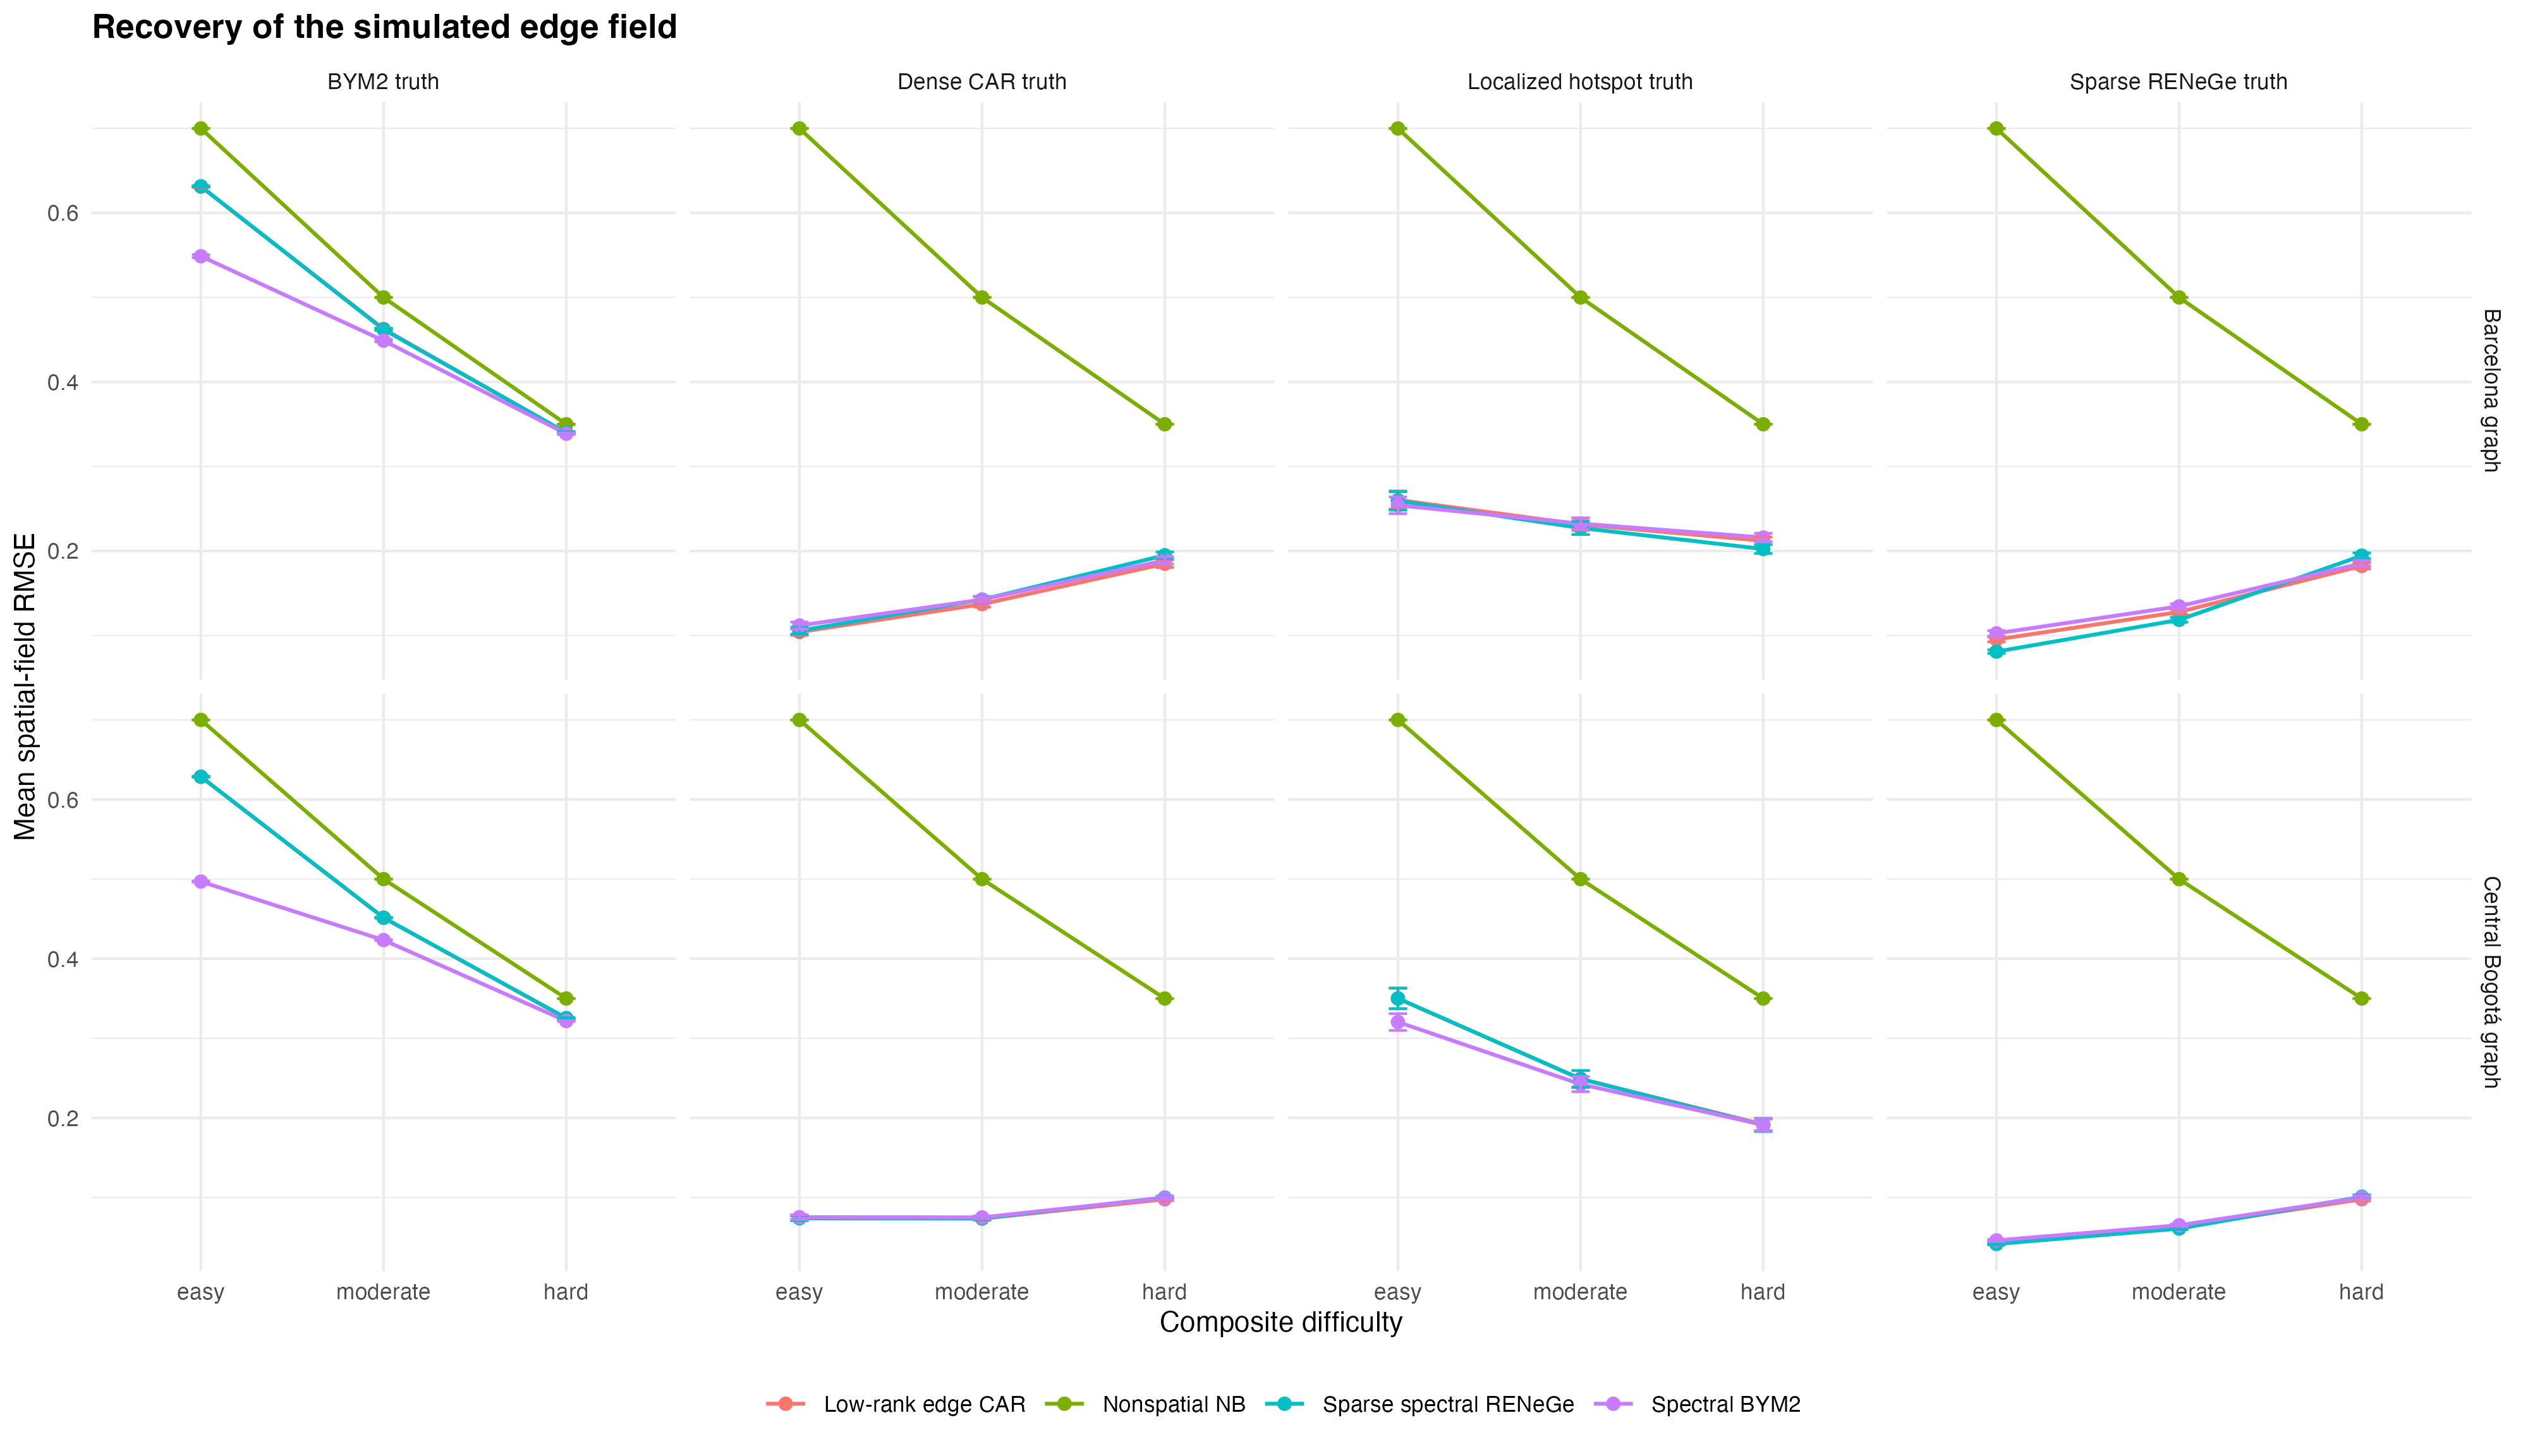
\includegraphics[width=\textwidth]{Fig04.png}
  \caption{Mean spatial-field RMSE across 50 replications for each network, generating mechanism, and composite difficulty level. Error bars are Monte Carlo standard errors. Lower values indicate better recovery}
  \label{fig:simulation-rmse}
\end{figure}

Predictive rankings were less separated among the three spatial models than field-recovery rankings (Fig.~\ref{fig:simulation-prediction}). Averaged across the 300 datasets generated under each truth, the proposed model improved mean test log score over the nonspatial model by 0.1442 under sparse RENeGe truth, 0.1215 under dense CAR truth, 0.1040 under hotspot truth, and 0.0186 under BYM2 truth. The corresponding paired Monte Carlo SEs were 0.0095, 0.0069, 0.0057, and 0.0010. These results show that a misspecified spatial basis can still predict substantially better than an independence model, but they do not imply that sparse selection dominates a correctly specified dense alternative.

\begin{figure}[!tbp]
  \centering
  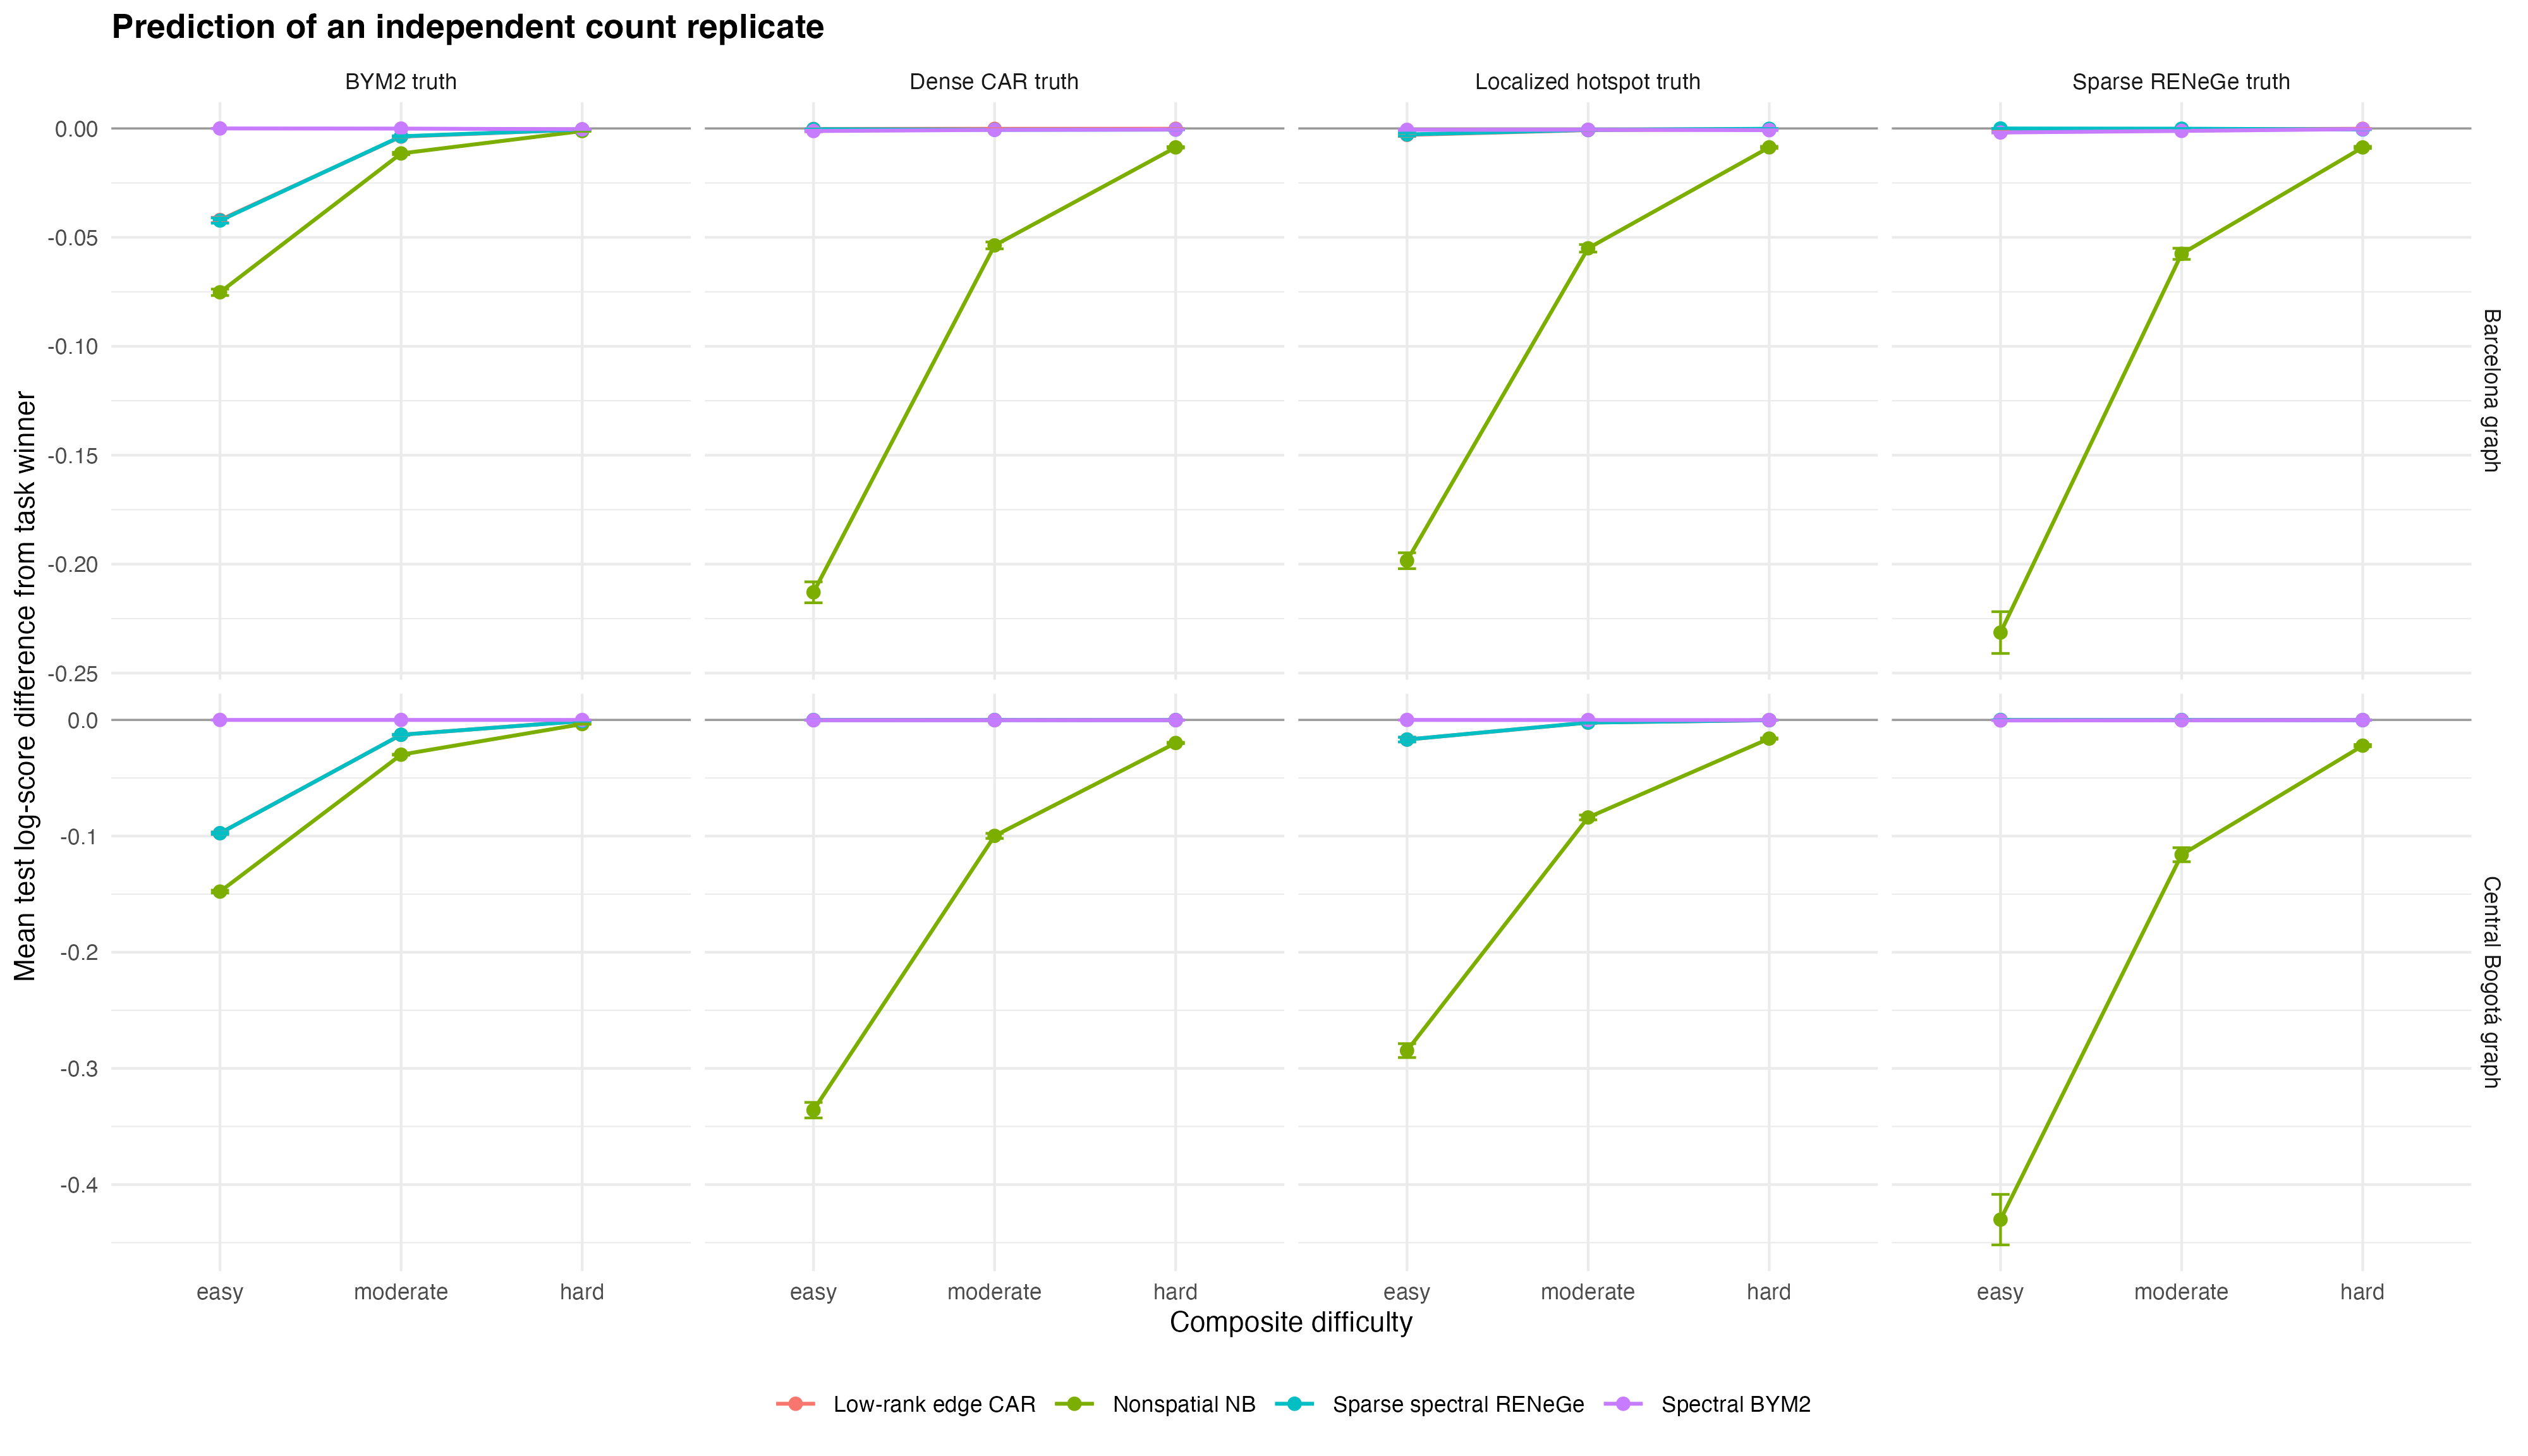
\includegraphics[width=\textwidth]{Fig05.png}
  \caption{Mean test log-score difference from the best model within each simulated dataset, evaluated on an independent count replicate. Zero denotes the task-specific winner; error bars are Monte Carlo standard errors}
  \label{fig:simulation-prediction}
\end{figure}

Recovery of active modes was strong when the sparse signal was identifiable (Table~\ref{tab:simulation-selection} and Fig.~\ref{fig:simulation-selection}). AUC was 1.00 in both networks under easy and moderate conditions, and the mean true-positive rate was at least 0.963 in the moderate condition. No inactive mode crossed the 0.5 classification threshold in any of the six aggregated cells, yielding zero false-discovery rate. In the hard condition, AUC remained 0.901 in Barcelona and 0.995 in Bogot\'a, but the true-positive rate fell to 0.068 and 0.168. The distinction between high ranking AUC and low threshold sensitivity indicates that the posterior remained able to order active modes while assigning probabilities conservatively when signal strength and intensity were reduced and the true active set increased to ten modes.

\begin{table}[!tbp]
  \centering
  \caption{Recovery of active modes by the proposed model under sparse RENeGe truth. Values are means over 50 replications. $K_0$ is the true number of active modes and $E(K\mid Y)$ is the posterior expected number.}
  \label{tab:simulation-selection}
  \begin{tabular}{llrrrrr}
    \toprule
    Network & Difficulty & $K_0$ & AUC & TPR & FDR & $E(K\mid Y)$ \\
    \midrule
    Barcelona & Easy & 3 & 1.000 & 1.000 & 0.000 & 3.48 \\
              & Moderate & 6 & 1.000 & 0.963 & 0.000 & 7.54 \\
              & Hard & 10 & 0.901 & 0.068 & 0.000 & 2.71 \\
    Central Bogot\'a & Easy & 3 & 1.000 & 1.000 & 0.000 & 3.42 \\
                     & Moderate & 6 & 1.000 & 0.997 & 0.000 & 7.58 \\
                     & Hard & 10 & 0.995 & 0.168 & 0.000 & 4.59 \\
    \bottomrule
  \end{tabular}
\end{table}

\begin{figure}[!tbp]
  \centering
  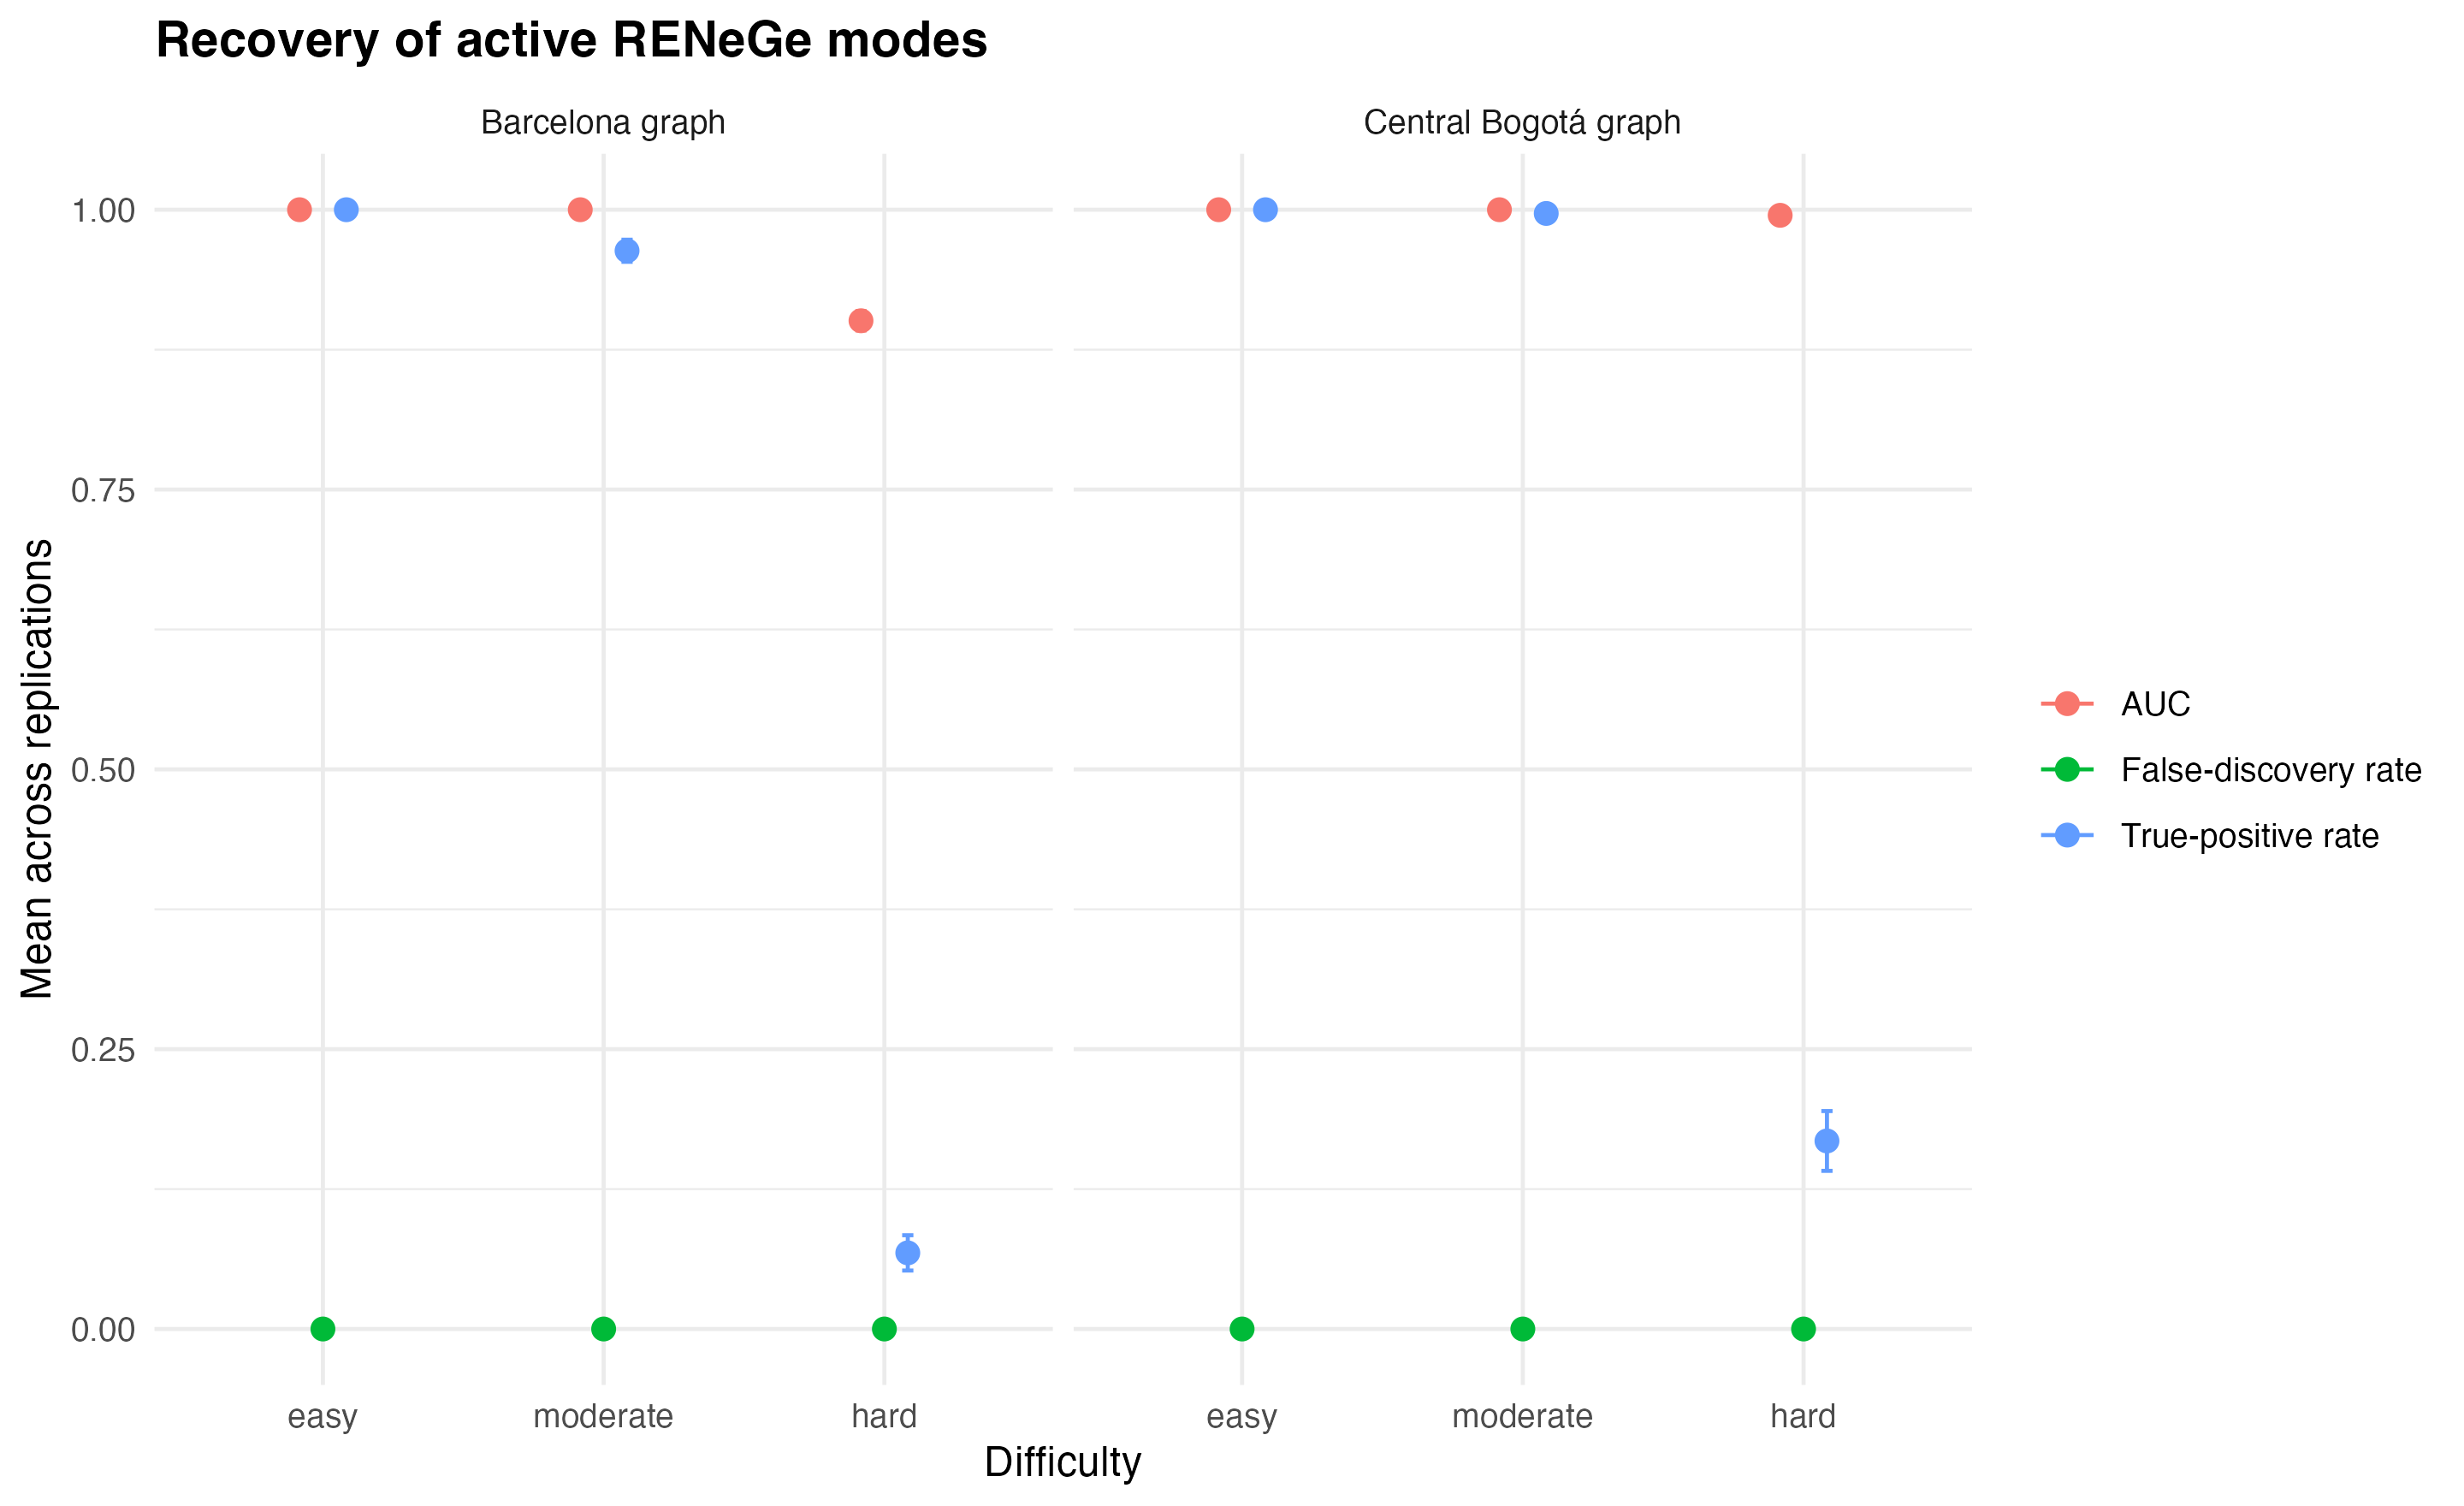
\includegraphics[width=0.88\textwidth]{Fig06.png}
  \caption{Mean AUC, true-positive rate, and false-discovery rate for mode recovery under sparse RENeGe truth. Error bars are Monte Carlo standard errors across 50 replications}
  \label{fig:simulation-selection}
\end{figure}

The simulation also exposed an important computational limitation (Table~\ref{tab:simulation-diagnostics}). Under the deliberately strict joint rule in Section~\ref{sec:simulation}, 90.3\% of proposed-model fits passed, compared with 67.0\% for low-rank CAR and 10.0\% for BYM2. The proposed model produced 105 divergent transitions in 69 of 1,200 fits; BYM2 produced 498 in 75 fits, including a maximum of 47 in one fit. CAR had no divergences, but its reported pass rate was only 67.0\%. The diagnostic rule above does not specify an $\widehat R$ cutoff; the aggregate summaries do not allow independent reconstruction of the reported pass classifications. BYM2's mean minimum bulk ESS was only 124, whereas the proposed model's was 1,295. Performance summaries retain all completed fits and must therefore be read together with these diagnostics.  

\begin{table}[!tbp]
  \centering
  \small
  \caption{Computational performance across 1,200 fits per model. Pass rate uses the joint diagnostic criterion defined above. Divergent fits counts fits with at least one divergence.}
  \label{tab:simulation-diagnostics}
  \resizebox{\textwidth}{!}{%
  \begin{tabular}{lrrrrr}
    \toprule
    Model & Pass (\%) & Divergent fits & Total diverg. & Mean min. ESS & Time (s) \\
    \midrule
    Sparse RENeGe & 90.3 & 69 & 105 & 1,295 & 16.6 \\
    Low-rank edge CAR & 67.0 & 0 & 0 & 336 & 24.5 \\
    Spectral BYM2 & 10.0 & 75 & 498 & 124 & 87.7 \\
    Nonspatial NB & 98.7 & 0 & 0 & 965 & 5.5 \\
    \bottomrule
  \end{tabular}%
  }
\end{table}

Within the legacy specification, these reported summaries support a targeted rather than universal claim; they do not establish performance of the revised prior. Sparse RENeGe is most useful when the network signal can be represented by a small subset of edge modes: it recovers the field accurately, ranks active components effectively, and preserves predictive performance relative to an unselected spectral CAR. When log-frequency contains substantial segment-specific variation, BYM2 can recover and predict better, but at the cost of weaker mode-level interpretation and, in this experiment, substantially more difficult posterior computation.






\section{Representative fields from the historical simulation}


\label{app:simulation-maps}

Figures~\ref{fig:simulation-map-barcelona} and~\ref{fig:simulation-map-bogota} visualize the four data-generating mechanisms on the two empirical network templates. To avoid selecting realizations by visual appearance, all panels use the preassigned replicate 25 from the moderate-difficulty condition. Within each network, the upper-row color scale is common across the four true latent fields, and the lower-row scale is common across the corresponding simulated training counts. The maps illustrate the broad, low-frequency structure of sparse RENeGe and dense CAR fields, the additional segment-level variation in BYM2, and the spatial concentration imposed by the localized-hotspot mechanism. They also show how negative-binomial sampling and heterogeneous segment exposure can partially obscure the latent structure in the observed counts.

\begin{figure}[!tbp]
  \centering
  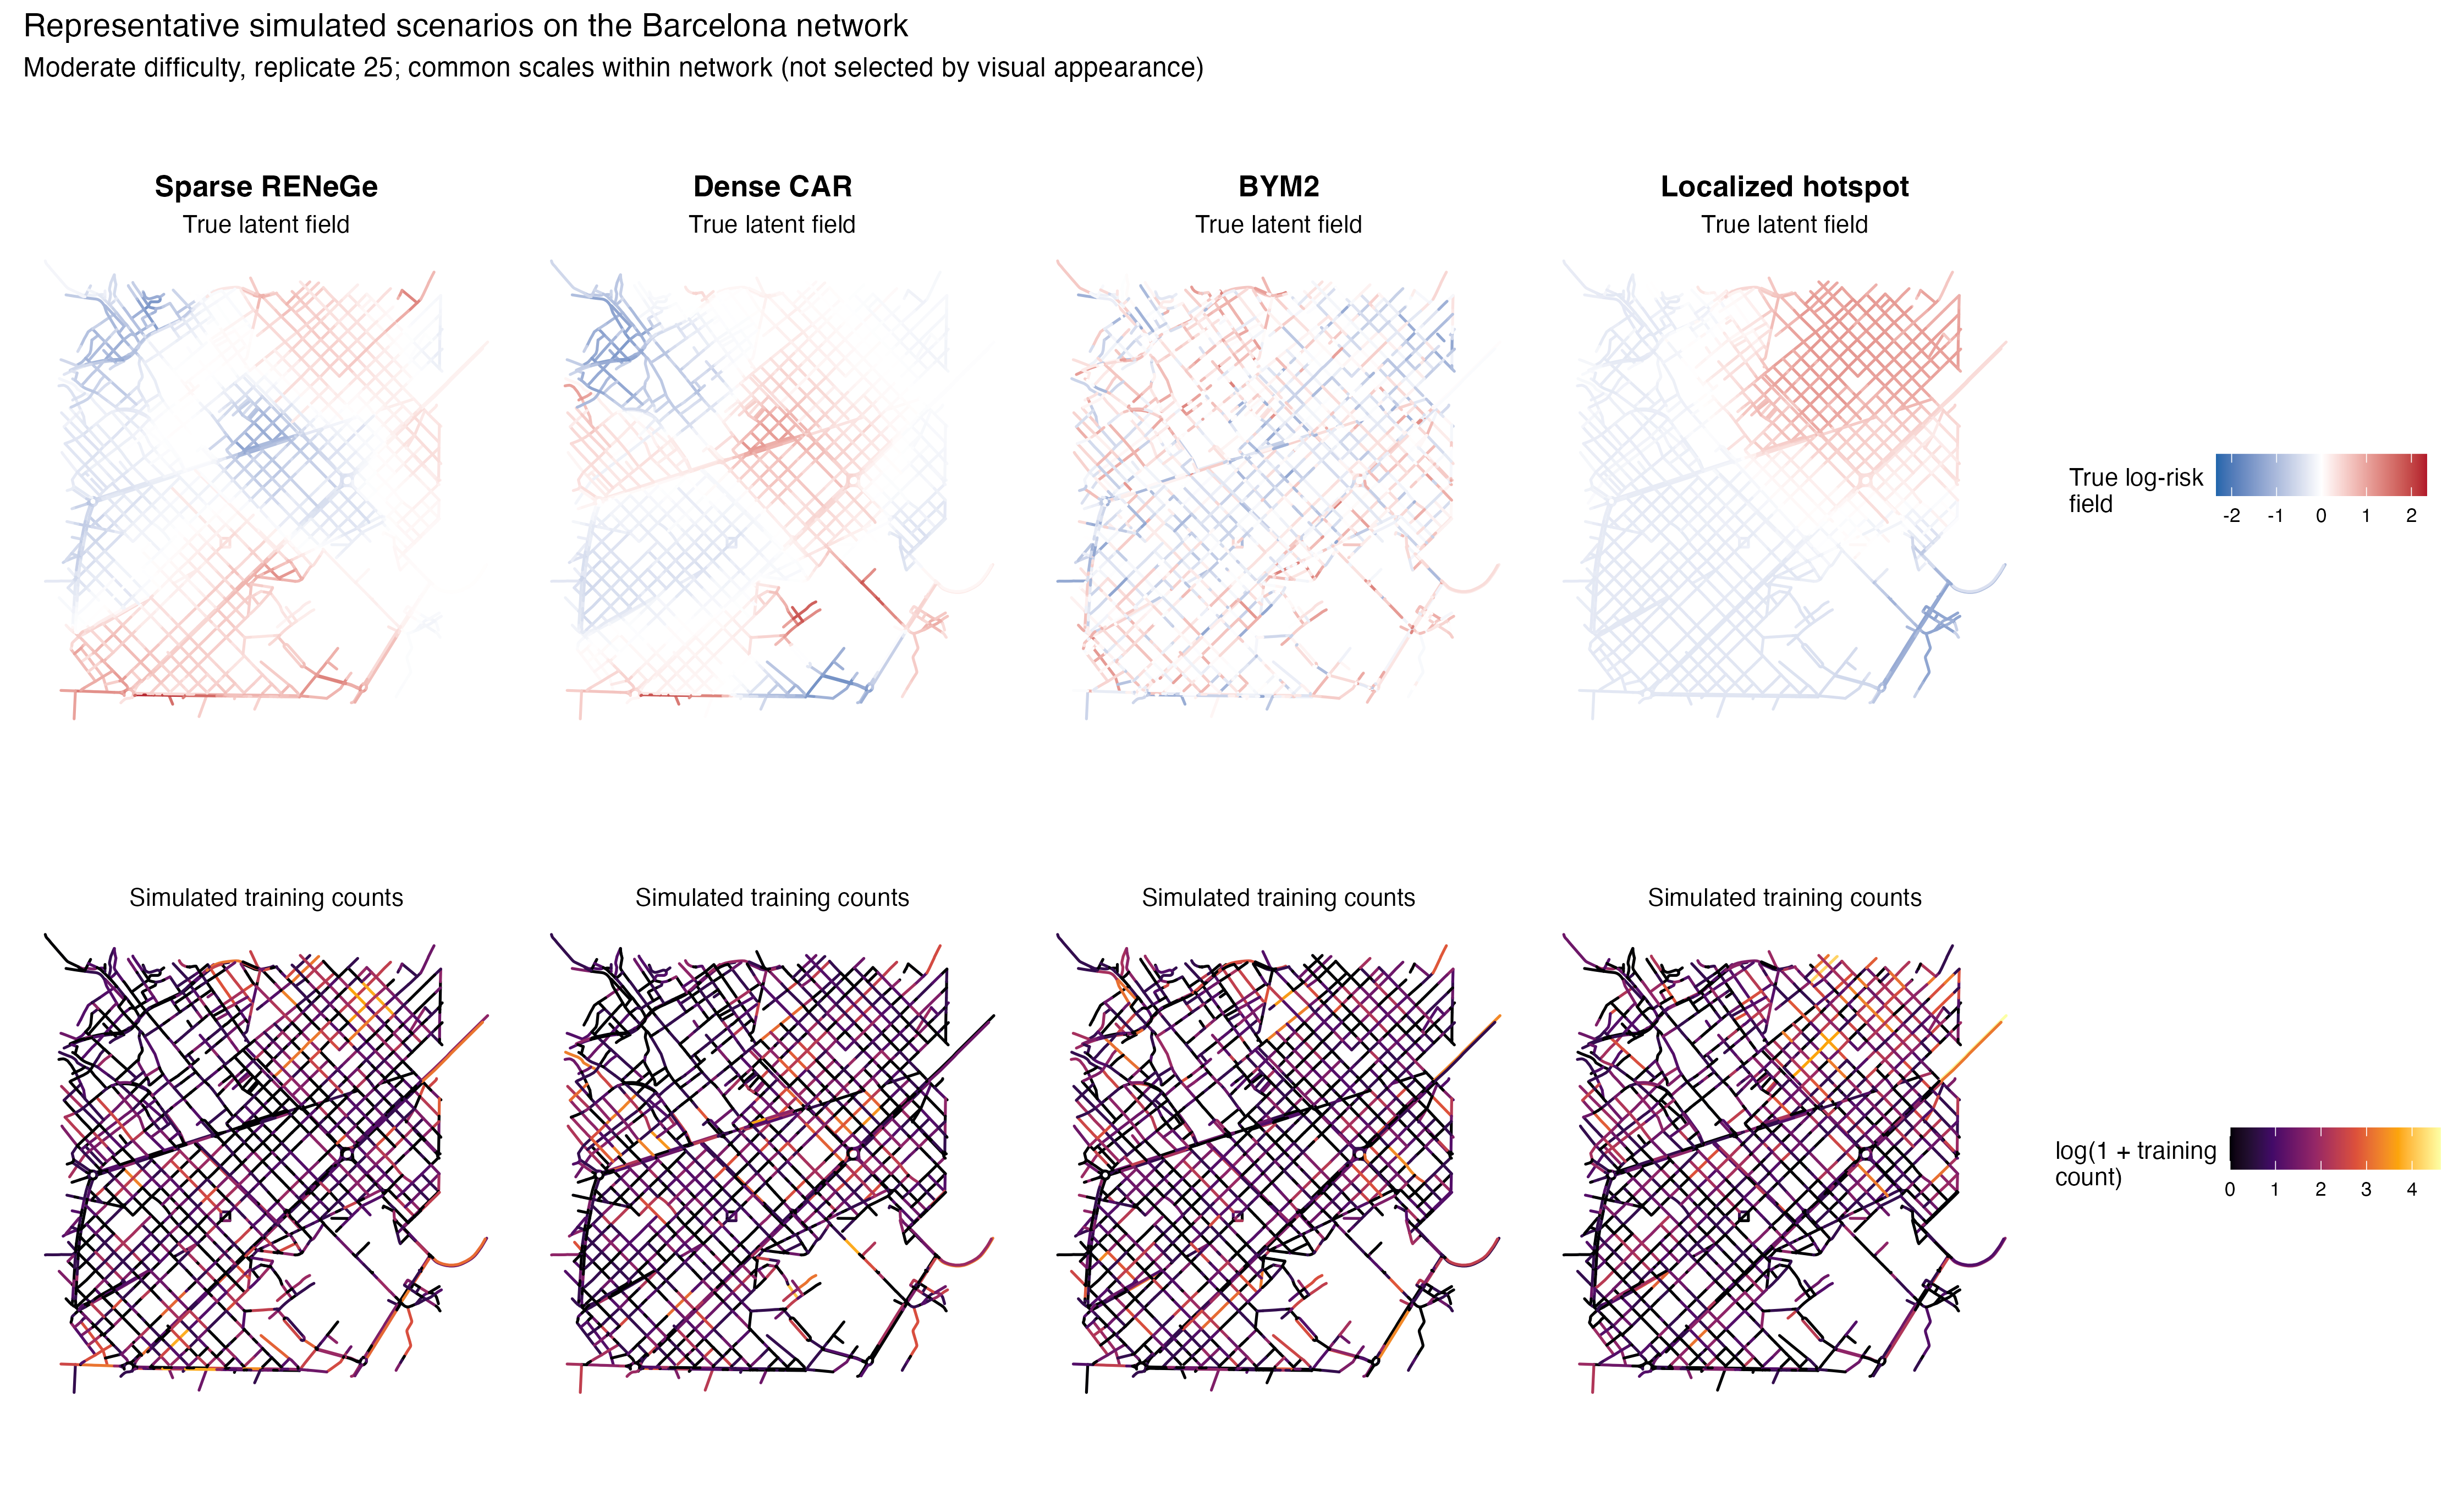
\includegraphics[width=\textwidth]{Fig16.png}
  \caption{Representative moderate-difficulty simulation on the Barcelona network. The upper row shows the true log-frequency field under each generating mechanism; the lower row shows the corresponding training counts on the log$(1+y)$ color scale. All panels use replicate 25}
  \label{fig:simulation-map-barcelona}
\end{figure}

\begin{figure}[!tbp]
  \centering
  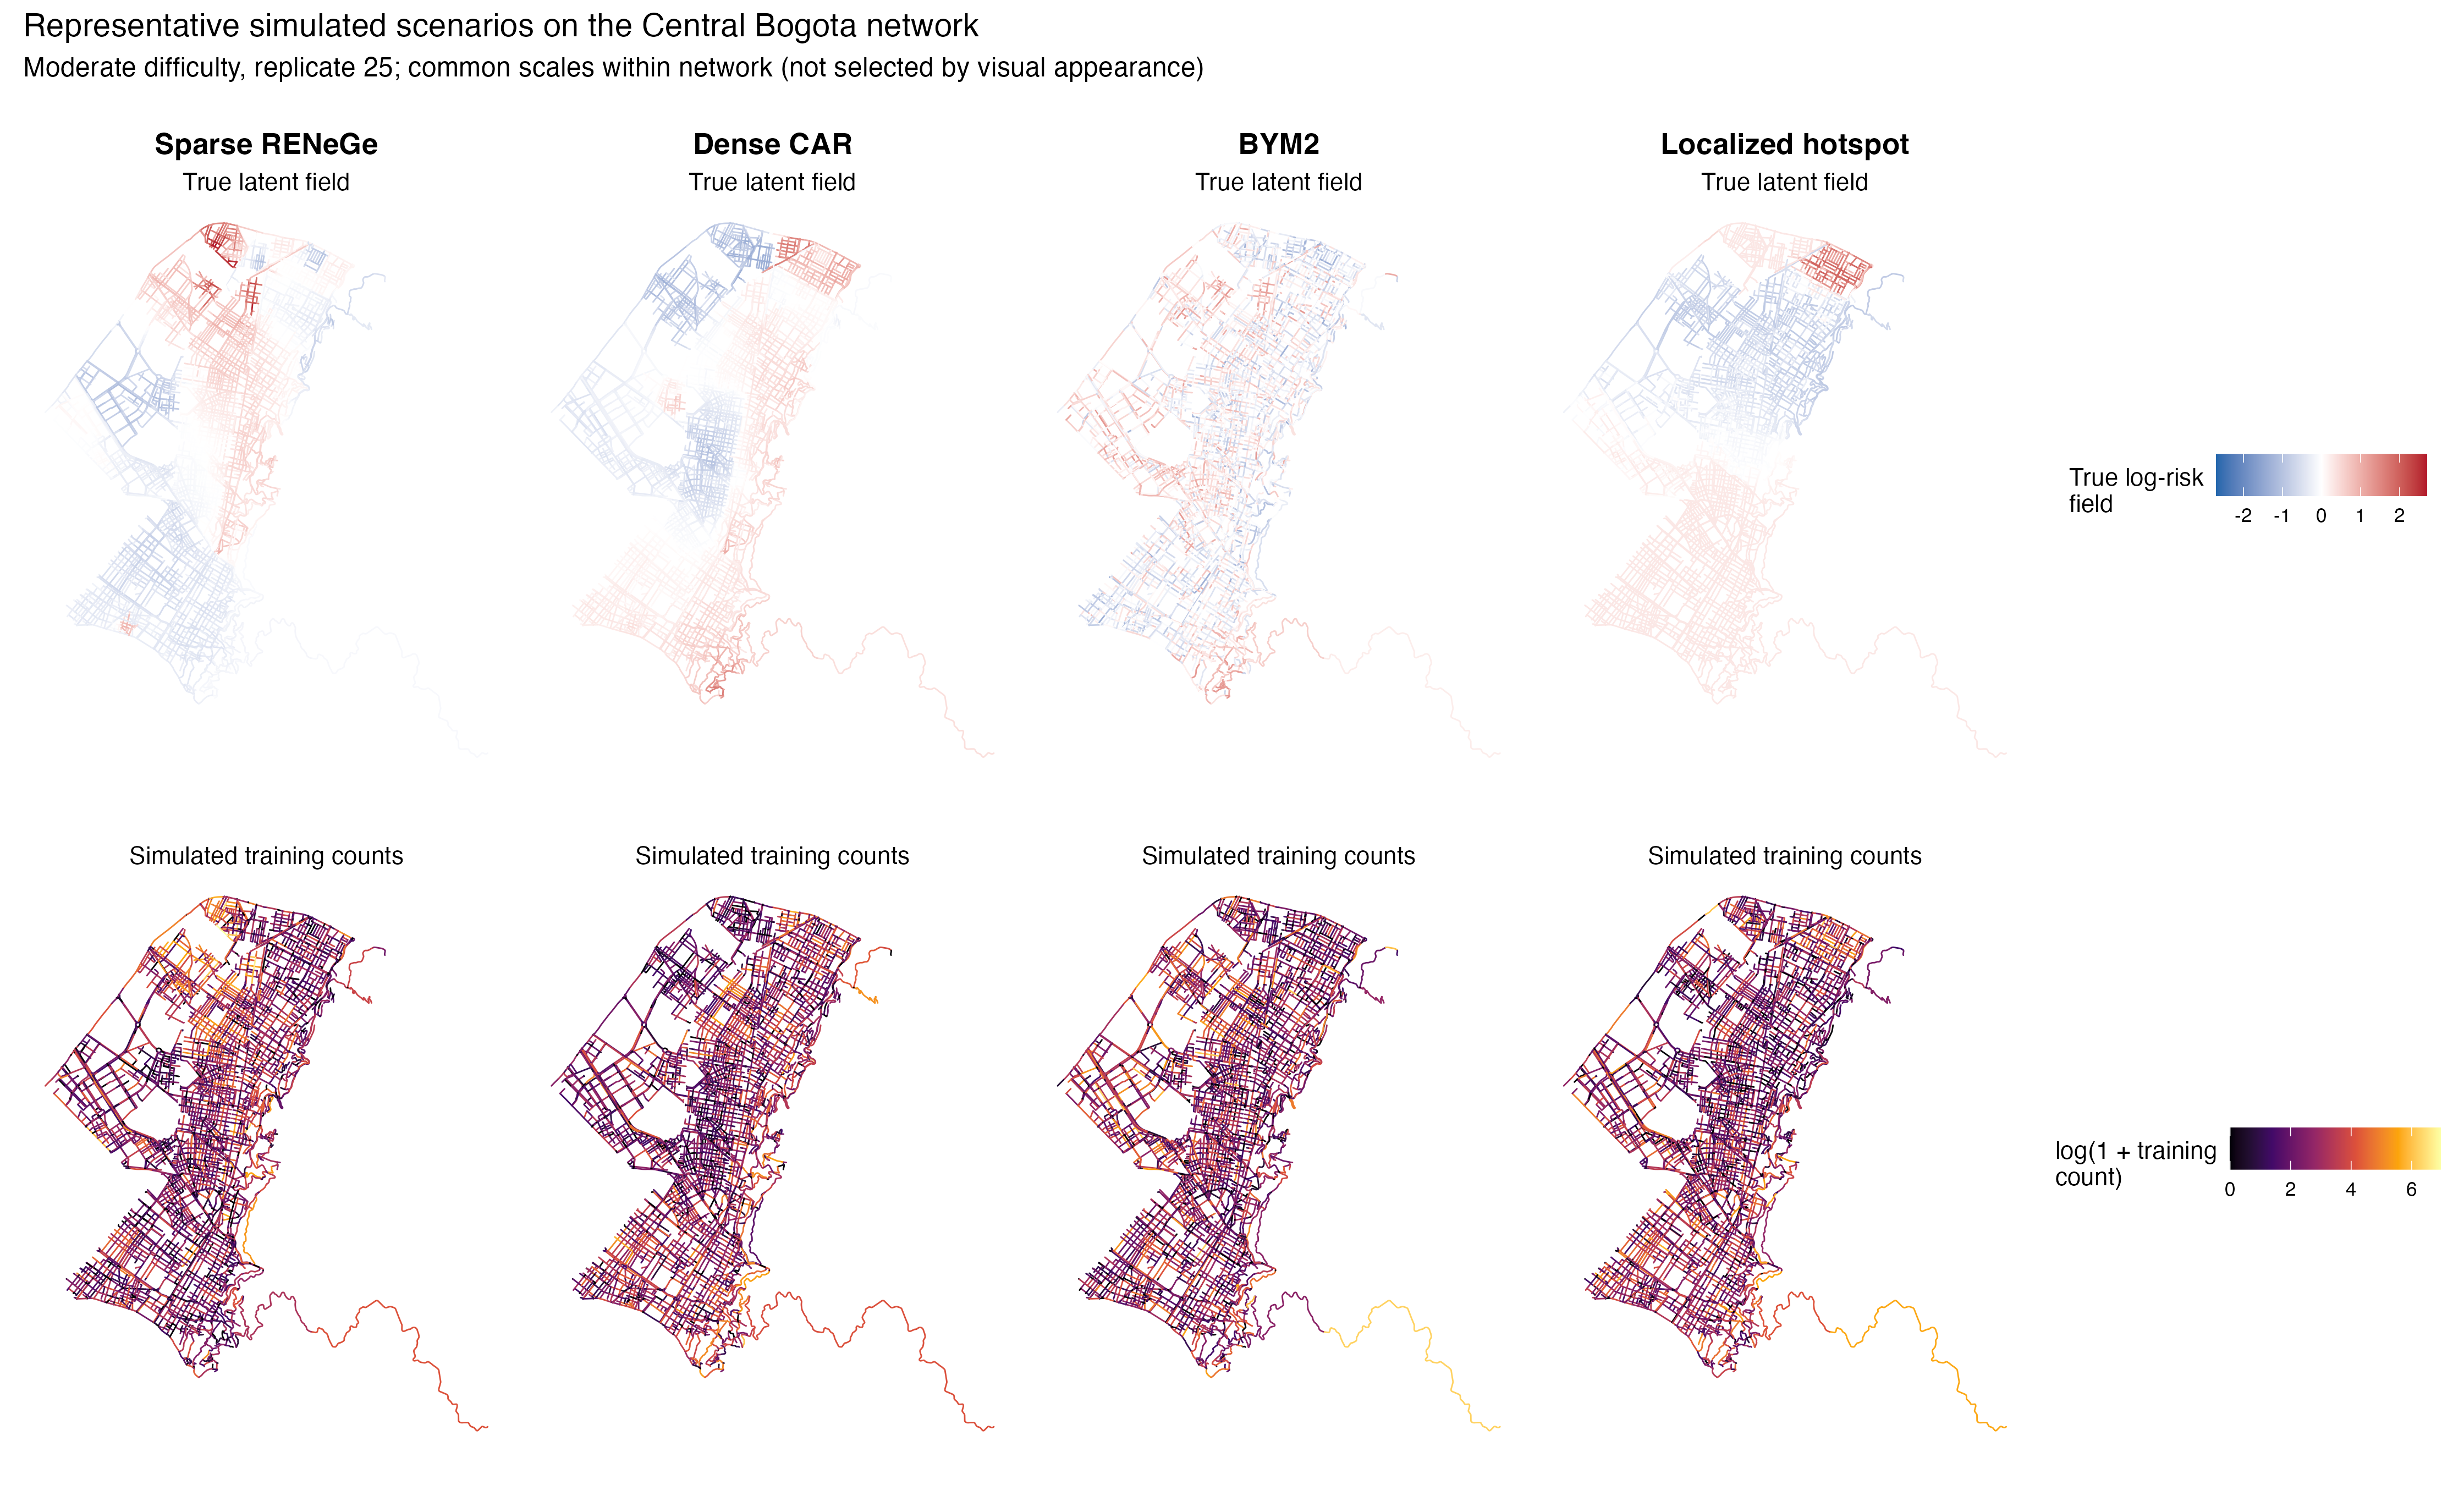
\includegraphics[width=\textwidth]{Fig17.png}
  \caption{Representative moderate-difficulty simulation on the central Bogot\'a network. The upper row shows the true log-frequency field under each generating mechanism; the lower row shows the corresponding training counts on the log$(1+y)$ color scale. All panels use replicate 25}
  \label{fig:simulation-map-bogota}
\end{figure}




\FloatBarrier



\FloatBarrier\end{document}